\section{Method}

We first will define a ground truth objective computable via brute and greedy algorithms that is uniquely minimized by orthonormal matrices.
We then define the combination of normalization and multitask basis pursuit that approximates this ground truth loss function.
We finally give a brute post-processing method for ensuring that the solution is $D$ sparse.

\subsection{Ground truth}
\label{sec:ground_truth}

The property of orthonormal matrices that motivates our ground truth loss function comes from spectral analysis.
\begin{proposition}[Singular values of a orthonormal matrix]
\label{prop:orthonormal_spectrum}
The singular values $\sigma_1 \dots \sigma_D$ are equal to $1$ if and only if $U \in \mathbb{R}^{D \times D}$ is orthonormal.
\end{proposition}

We'd like a ground truth objective to be minimized uniquely by orthonormal matrices, invariant under rotation, and depend on all changes in the matrix.
The first desired property precludes, for example, the log determinant, while the last precludes the the deformation. %check
Finally, to simplify our overall exposition and exemplify the key features of the method, we'd like this ground truth loss to be as similar as possible to the convex loss we introduce.

Thus, we define the loss
\begin{align}
l_{c}: \mathbb R^{D \times P} \to \mathbb R^{+} \\
\mathcal X \mapsto \sum_{d = 1}^D g(\sigma^d(\mathcal X), c)
\end{align}
where $\sigma^d (\mathcal (X))$ is the $d$-th singular value of $\mathcal X$ and
\begin{align}
g: \mathbb R^+ \times \mathbb R^+ &\to \mathbb R^+ \\
t,c &\mapsto e^{t^c} + e^{t^{-c}}.
\end{align}
Plainly, $g$ is uniquely maximized by orthonormal matrices, and $g(\mathcal X^{\dagger}) = g(\mathcal X)^{-1}$.
The former condition is necessary for success of the method, while the latter, as well as the convexity of $g$, are somewhat aesthetic choices.
A graph of $g$ is given in Figure \ref{fig:gt_loss}.
Most importantly, this loss enables comparison with produced after normalization as in Section \ref{sec:normalization}.
%This loss is an appropriate choice for comparison because it is equal to the basis pursuit loss for suitably normalized orthogonal matrices.

% NOTE (Sam): this could be improved.  Do we need proofs of maximized by orthonormal matrices and convex?
% Something like the justification for logarithmic symmetry would be useful here.
% Why do we need convex here? Convex functions form metric? Cite Koelle neuroscience? Is metric important?
% Can we prove this is a norm?

\begin{align}
\label{prog:ground_truth}
\widehat {\mathcal S}_{GT}  &= \arg \min_{\mathcal S \subseteq [P] : |\mathcal S| = D} l_c (\mathcal X_{.\mathcal S})
\end{align}

Regardless of the convexity of $l_c$, brute combinatorial search over $[P]$ is inherently non-convex.

\subsection{Normalization}
\label{sec:normalization}

Since basis pursuit methods tend to select longer vectors, selection of orthonormal submatrices requires normalization such that both long and short candidate basis vectors are penalized in the subsequent regression, we make the following definition.

\begin{definition}[Symmetric normalization]
% NOTE (Sam): need a better name for this type of function.  Can I reuse parts in ground truth section?  Keep in mind max/min is switched).
A function $q: \mathbb R^D \to \mathbb R^+ $ is a symmetric normalization if 
\begin{align}
\arg \max_{v \in \mathbb R^D} \ q (v) &=\{ v : \|v\| = 1 \} \\
q(v) &= q(\frac{v}{\|v\|^2}) \\
q(v^1) &= q(v^2) \; \forall \; v^1, v^2 : \|v^1\| = \|v^2\|
\end{align}
\label{def:symmetric_normalization}
\end{definition}

Normalization by functions satisfying this definition is sufficient for the application of multitask basis pursuit for finding isometries.
The vectors are in particular length normalized so that the post-normalization vectors with the longest length correspond to pre-normalization vectors of length $1$.
We therefore propose the following normalization.

\begin{align}
\label{eq:normalization}
% Note (Sam): fix this... get and more ... q_c?
q: \mathbb R^+ \times \mathbb R^+  &\to \mathbb R^+ \\
t , c &\mapsto \frac{e^{t^c} + e^{t^{-c}}}{2e},
\end{align}
and use this to define the vector normalization 
\begin{align}
n: \mathbb R^D \times \mathbb R^+ &\to \mathbb R^D \\
n , c &\mapsto \frac{n}{q(\|n\|_{2},c) }
\end{align}
and matrix normalization
\begin{align}
w: \mathbb R^{D \times P} \times \mathbb R^+ &\to \mathbb R^D \\
\mathcal X_{.p} , c &\mapsto n(\mathcal X_{.p}, c) \; \forall \; p \in [P].
\end{align}

Besides satisfying the conditions in Definition \ref{def:symmetric_normalization}, this normalization has some additional nice properties.
First, $q$ is convex.
Second, it grows asymptotically log-linearly.
Third, while $\exp(-|\log t|) = \exp(-\max (t, 1/t))$ is a seemingly natural choice for normalization, it is non smooth, and the LogSumExp replacement of $\max (t, 1/t)$ with $ \log (\exp (t ) + \exp(1/t))$ simplifies to \ref{eq:normalization} upon exponentiation \citep{Boyd2004-ql}.
Finally, the parameter $c$ grants control over the width of the basin, which is important in avoiding numerical issues arising close to $0$ and $\infty$.

\begin{figure}
\centering
\subcaptionbox{Ground truth loss scaling function $g$ as a function of $t$. \label{cat}}
{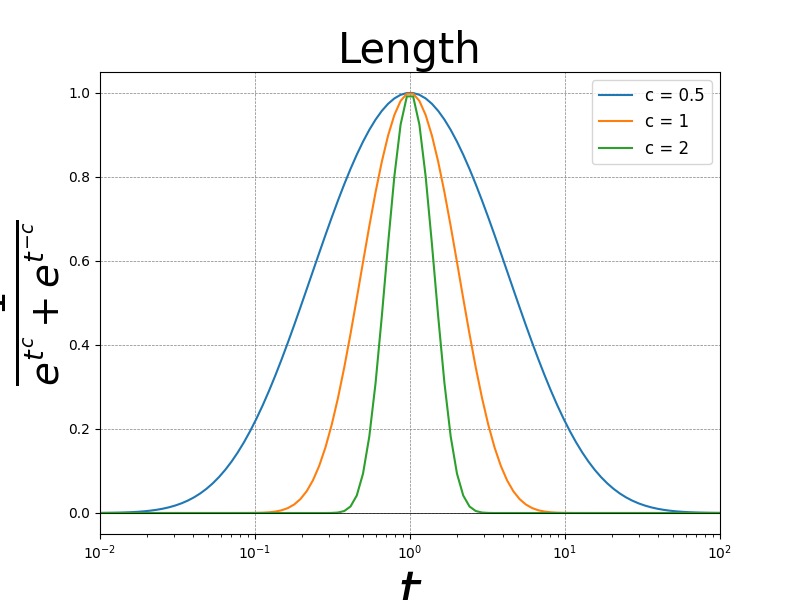
\includegraphics[width = .33\textwidth]{../figures/Figure_1a.png}}
\subcaptionbox{Length as a function of $t$ \label{elephant}}
{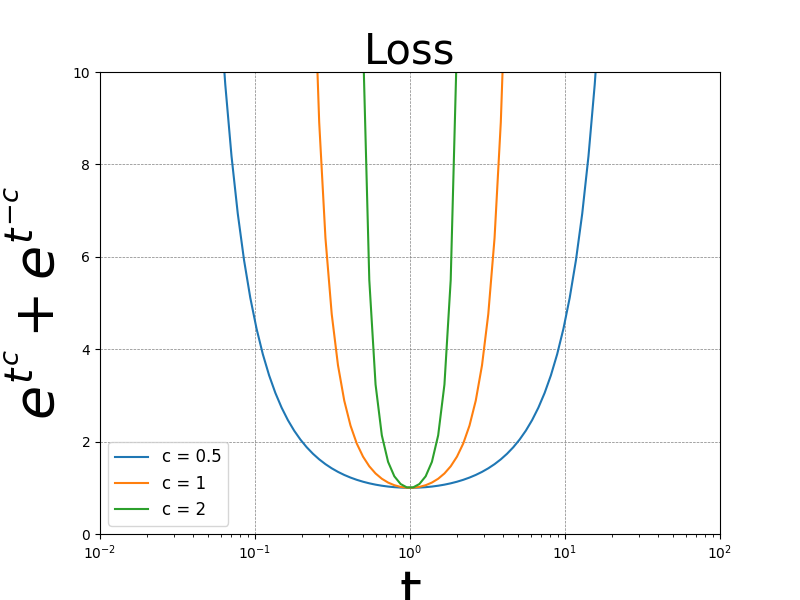
\includegraphics[width = .33\textwidth]{../figures/Figure_1b.png}}
\caption{Plots of Length and Loss for different values of $c$.
   Since $t$ is one dimensional and therefore diagonalizable, basis pursuit and ground truth give identical loss values.}\label{animals}
\end{figure}

\subsection{Isometry pursuit}

Isometry pursuit is the application of multitask basis pursuit to the appropriate normalized design matrix $w(\mathcal X)$ to identify submatrices of $\mathcal X$ that are as orthonormal as possible.
Define the multitask basis pursuit penalty 
\begin{align}
\label{eq:bp}
\| \cdot \|_{1,2}: \mathbb R^{P \times D} &\to \mathbb R^+ \\ 
\beta &\mapsto  \sum_{p=1}^P  \|\beta_{p.}\|_2.
\end{align}
The isometry pursuit program is then
\begin{align}
\label{prog:isometry_pursuit}
\widehat \beta^{D}_c (\mathcal X)  := \arg \min_{\beta \in \mathbb R^{P \times D}} \| \beta \|_{1,2} \; : \; I_D = w ({ \mathcal X}, c) \beta.
\end{align}
The recovered functions are the indices of the dictionary elements with non-zero coefficients.
That is, they are given by $S(\beta)$ where 
\begin{align}
S: \mathbb{R}^{p \times d} &\to \binom{[P]}{d} \\
\beta &\mapsto \left\{ p \in [P] :  \|\beta_{p.}\| > 0 \right\}
\end{align}
and $\binom{[P]}{d} = \left\{ A \subseteq [P] : \left|A\right| = d \right\}$. 
\begin{algorithm}[H]
\caption{\texttt{IsometryPursuit}(Matrix $\mathcal{X} \in \mathbb{R}^{D \times P}$, scaling constant $c$)}
\begin{algorithmic}[1]
\STATE {\bf Output} $\widehat{S} = S (\widehat{\beta}_P(w_c(\mathcal{X})))$
\end{algorithmic}
\end{algorithm}

A key initial theoretical assertion for the feasibility of \isometrypursuit~ is that it is invariant to choice of basis for $\mathcal X$.
\begin{proposition}[Basis pursuit selection invariance]
\label{prop:basis_pursuit_selection_invariance}
Let $U \in \mathbb R^{D \times D}$ be orthonormal.
 Then $S(\widehat \beta  (U \mathcal X)) = S(\widehat \beta (\mathcal X))$.
\end{proposition}
A proof is given in Section \ref{proof:basis_pursuit_program_invariance}
This fact has as an immediate corollary that we may replace $I_D$ in the constraint by any orthonormal $D \times D$ matrix.

The intuition behind our application of multitask basis pursuit in our setting is that submatrices consisting of vectors which are closer to 1 in length and more orthogonal will have smaller loss.
The property of orthonormal matrices that corresponds to this is slightly different from Proposition \ref{prop:orthonormal_spectrum}.
\begin{proposition}[Basis vectors of a orthonormal matrix]
\label{prop:orthonormal_basis}
The component vectors $u^1 \dots u^D \in \mathbb R^B$ form a orthonormal matrix if and only if, for all $d_1, d_2 \in [D], u_{d_1} u^{d_2} = \begin{cases}
1 \; d_1 = d_2\\ 
0 \; d_1 \neq d_2 
\end{cases}$.
\end{proposition}
We show theoretically that the conditions of the consequent of Proposition \ref{prop:orthonormal_basis} are satisfied by minimizers of the multitask basis pursuit objective applied to suitably normalized matrices in the special case where both such a submatrix exists and $|\mathcal S| = D$.
\begin{proposition}[Unitary preference]
Let $w_c$ be a normalization satisfying the conditions in Definition \ref{eq:symmetric_normalization}.  Then $\arg \min_{X_{.S} \in \mathbb R^{D \times D}} \widehat \beta^{D}_c (\mathcal X) $ is orthonormal.  Moreover when $X$ is orthonormal, $\min_{\beta \in \mathbb R^{P \times D}} \| \beta \|_{1,2} \; : \; I_D = w ({ \mathcal X}, c) \beta = D$.
\label{prop:unitary_selection}
\end{proposition}
While this Proposition falls short of showing that an orthonormal submatrix will be selected should one be present, it provides intuition justifying the preferential efficacy of Isometry Pursuit on real data.

\subsection{Two-stage isometry pursuit}

Since cannot in general ensure either that $|\widehat { \mathcal S|} = D$ or that a orthonormal submatrix $X_{.S}$ exists, we apply a standard approach in the lasso literature: to first use the convex problem to prune, prior to a final feature selection step \cite{Hesterberg2008-iy}.
For simplicity, we propose using brute selection applied to the estimated feature set $\widehat S$.
In practice, this 

\begin{algorithm}[H]
\caption{\texttt{TwoStageIsometryPursuit}(Matrix $\mathcal{X} \in \mathbb{R}^{D \times P}$, scaling constant $c$, objective $f$)}
\begin{algorithmic}[1]
\STATE $\widehat{S_1} = \texttt{IsometryPursuit}(\mathcal X, c)$
\STATE $\widehat{S} = \texttt{Brute}(\mathcal{X}_{.\widehat{S_1}}, f)$
\STATE {\bf Output} $\widehat{S}$
\end{algorithmic}
\end{algorithm}


%\subsection{Implementation}


%\subsection{Computational complexity}
%\label{sec:computation_complexity}
